\documentclass{beamer}

\usefonttheme{professionalfonts} % using non standard fonts for beamer
\usefonttheme{serif} % default family is serif

\usepackage{enumitem}
\setitemize{label=\usebeamerfont*{itemize item}%
  \usebeamercolor[fg]{itemize item}
  \usebeamertemplate{itemize item}}

\usepackage{hyperref}
%\usepackage{minted}
\usepackage{animate}
\usepackage{graphicx}
\def\Put(#1,#2)#3{\leavevmode\makebox(0,0){\put(#1,#2){#3}}}
\usepackage{colortbl}
\usepackage{tikz}
\usepackage{amssymb}
\usepackage{enumerate}
\usepackage{arydshln}
\usepackage{algorithm}
\usepackage{algpseudocode}

\usepackage[absolute,overlay]{textpos}

\colorlet{lightred}{red!25}
\colorlet{lightgreen}{green!25}
\beamertemplatenavigationsymbolsempty

\newcommand\blfootnote[1]{%
  \begingroup
  \renewcommand\thefootnote{}\footnote{#1}%
  \addtocounter{footnote}{-1}%
  \endgroup
}

\makeatletter

%% Textclass specific LaTeX commands.
\newcommand\makebeamertitle{\frame{\maketitle}}%
\AtBeginDocument{%
  \let\origtableofcontents=\tableofcontents
  \def\tableofcontents{\@ifnextchar[{\origtableofcontents}{\gobbletableofcontents}}
  \def\gobbletableofcontents#1{\origtableofcontents}
}
%% User specified LaTeX commands.
\usetheme{Malmoe}
\useoutertheme{infolines}
\addtobeamertemplate{headline}{}{\vskip2pt}
\setbeamercovered{transparent}

\makeatother

%%%%%%%%%%%%%%%%%%%%%%%%%%%%%%%%%%%%%%
%% Main document
%%%%%%%%%%%%%%%%%%%%%%%%%%%%%%%%%%%%%%
\begin{document}
\title[PFLOCK report]{PFLOCK Report}
\author[AC]{Andres Calderon}
\institute[Fall'20]{University of California, Riverside}
\makebeamertitle
\newif\iflattersubsect

\AtBeginSection[] {
    \begin{frame}<beamer>
    \frametitle{Outline} 
    \tableofcontents[currentsection]  
    \end{frame}
    \lattersubsectfalse
}

\AtBeginSubsection[] {
    \begin{frame}<beamer>
    \frametitle{Outline} 
    \tableofcontents[currentsubsection]  
    \end{frame}
}

\begin{frame}{Welzl's algorithm...}{Foundation}
    \centering
    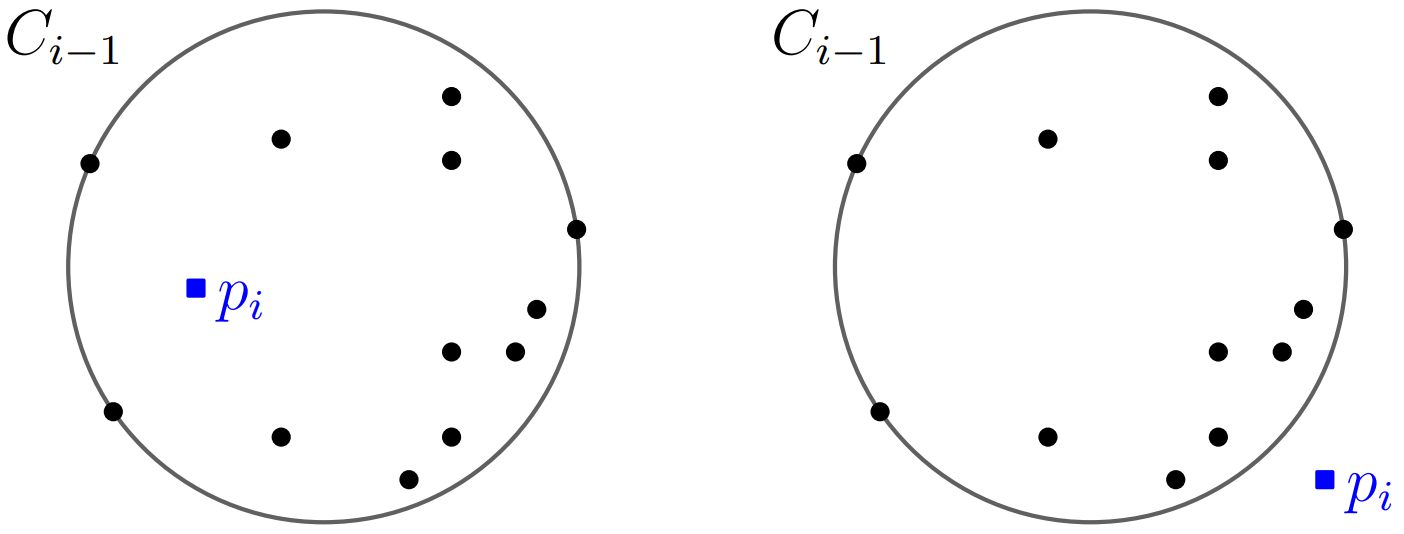
\includegraphics[width=0.9\textwidth]{figures/foundation} 
\end{frame}

\begin{frame}{Welzl's algorithm...}{Example}
    \centering
    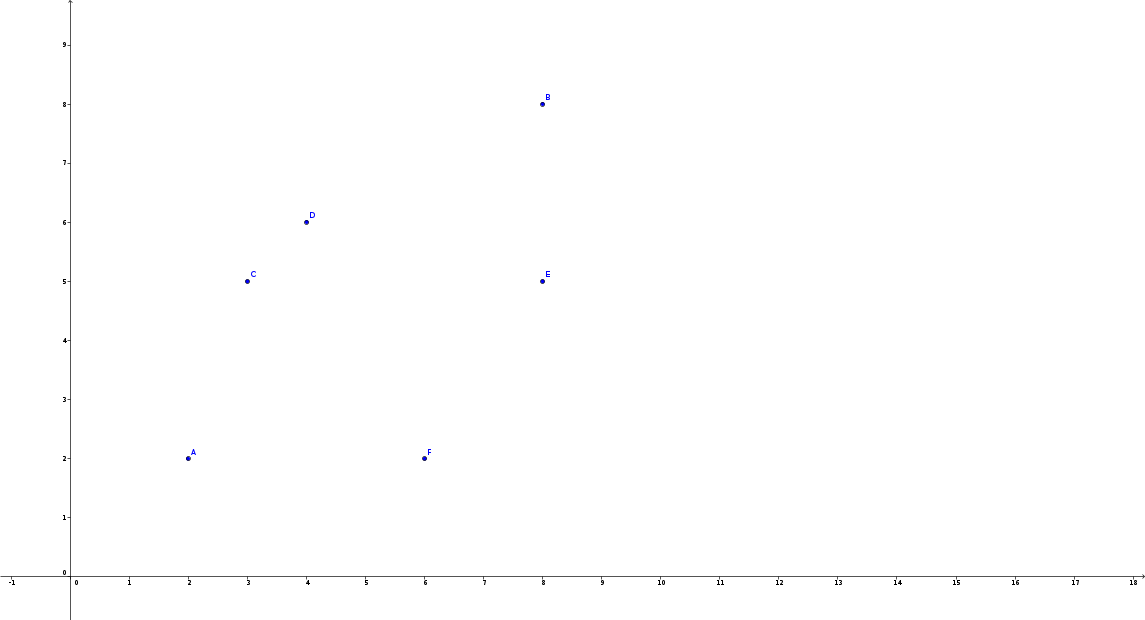
\includegraphics[trim=0 0 7cm 0,clip,width=0.65\textwidth]{figures/SEC01} \\
    $P = \{C, D, E, F, A, B\}$
\end{frame}
\begin{frame}{Welzl's algorithm...}{Example}
    \centering
    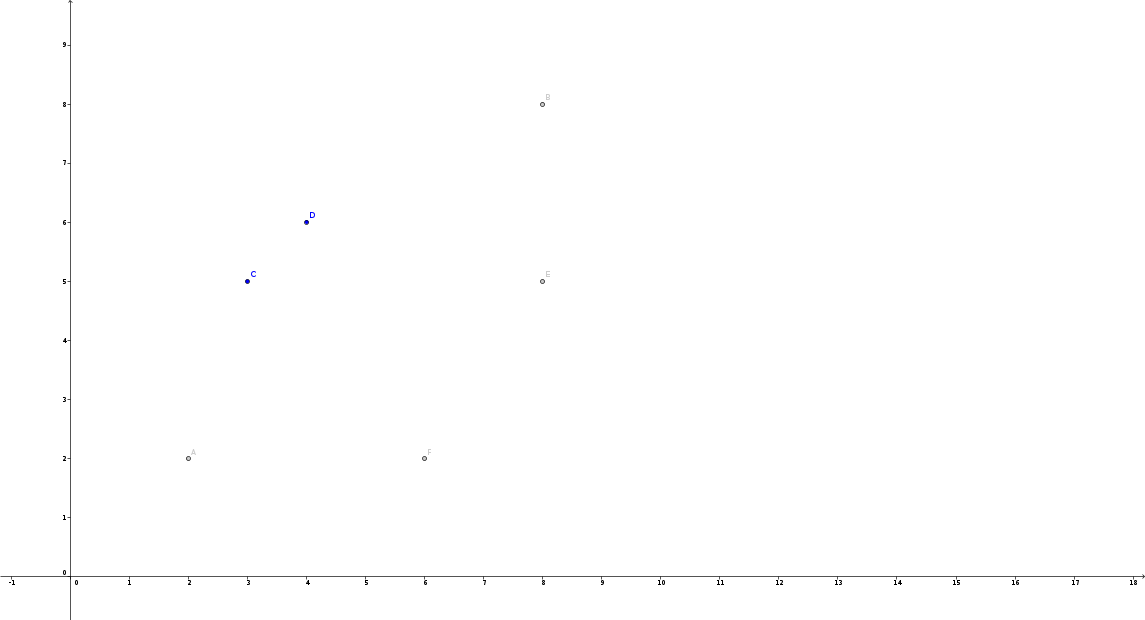
\includegraphics[trim=0 0 7cm 0,clip,width=0.65\textwidth]{figures/SEC02} \\
    $P = \{C, D, E, F, A, B\}$
\end{frame}
\begin{frame}{Welzl's algorithm...}{Is next point inside the current disk?}
    \centering
    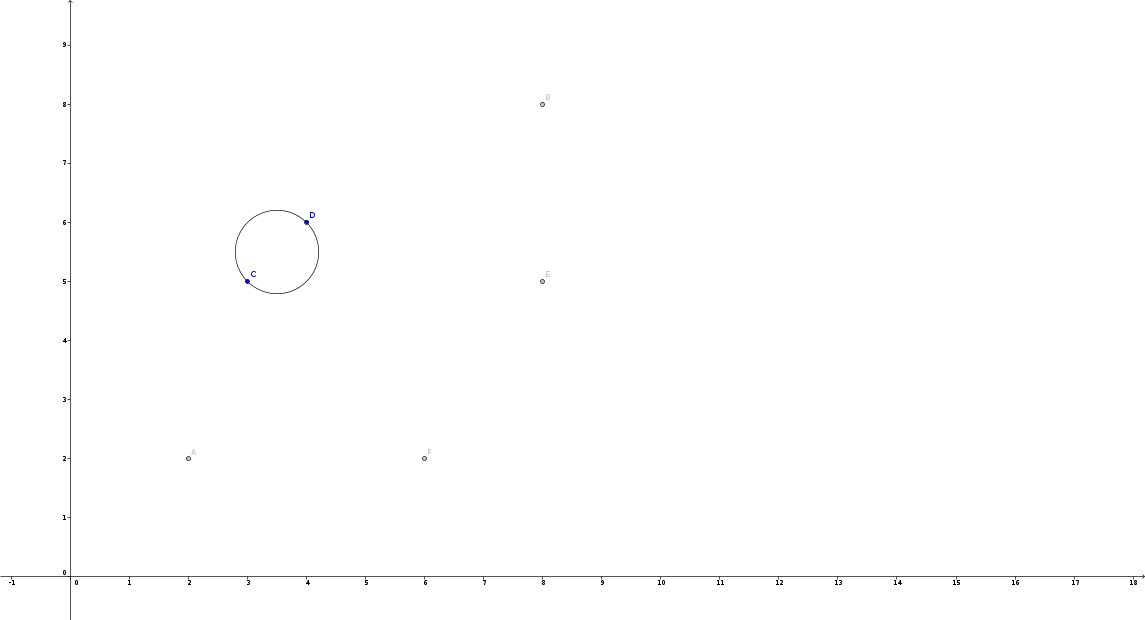
\includegraphics[trim=0 0 7cm 0,clip,width=0.65\textwidth]{figures/SEC03} \\
    $P = \{C, D, \mathbf{E}, F, A, B\}$
\end{frame}
\begin{frame}{Welzl's algorithm...}{Now new point must be in the boundary and Move To The Front heuristic...}
    \centering
    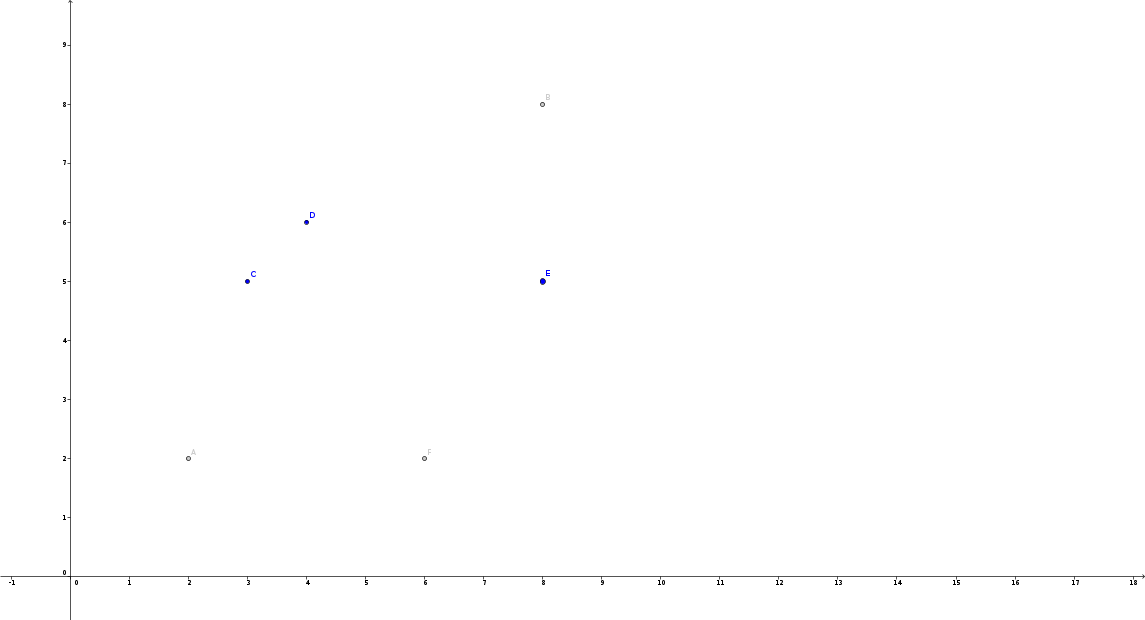
\includegraphics[trim=0 0 7cm 0,clip,width=0.65\textwidth]{figures/SEC04} \\
    $P = \{E, C, D, F, A, B\}$
\end{frame}
\begin{frame}{Welzl's algorithm...}{Repeat the process for subsequent points...}
    \centering
    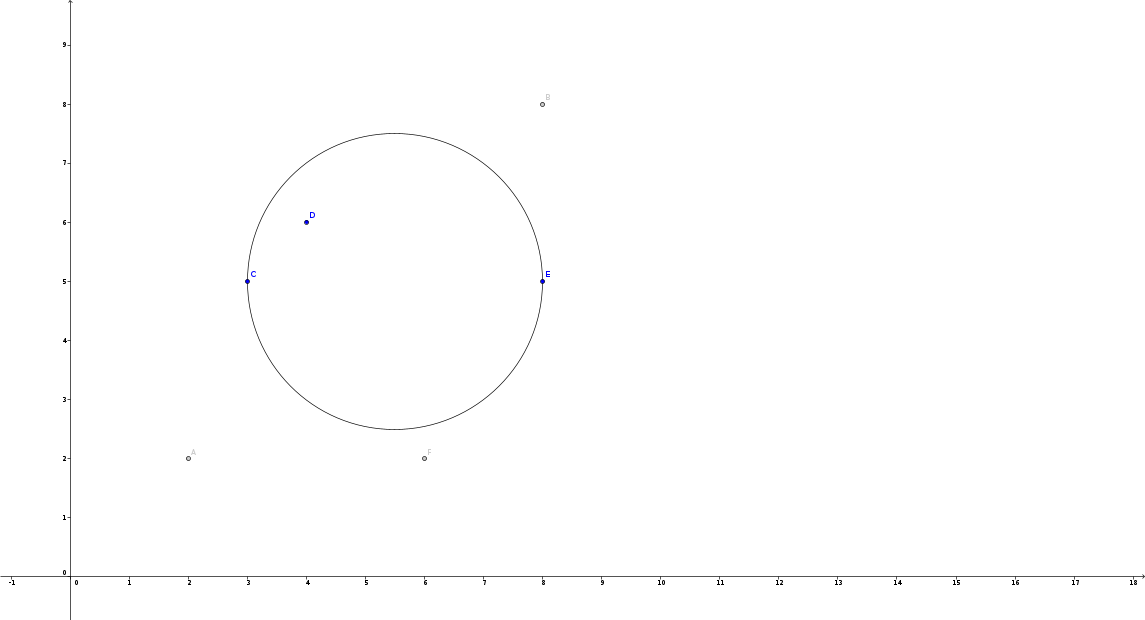
\includegraphics[trim=0 0 7cm 0,clip,width=0.65\textwidth]{figures/SEC05} \\
    $P = \{E, C, D, F, A, B\}$
\end{frame}
\begin{frame}{Welzl's algorithm...}{Repeat the process for subsequent points...}
    \centering
    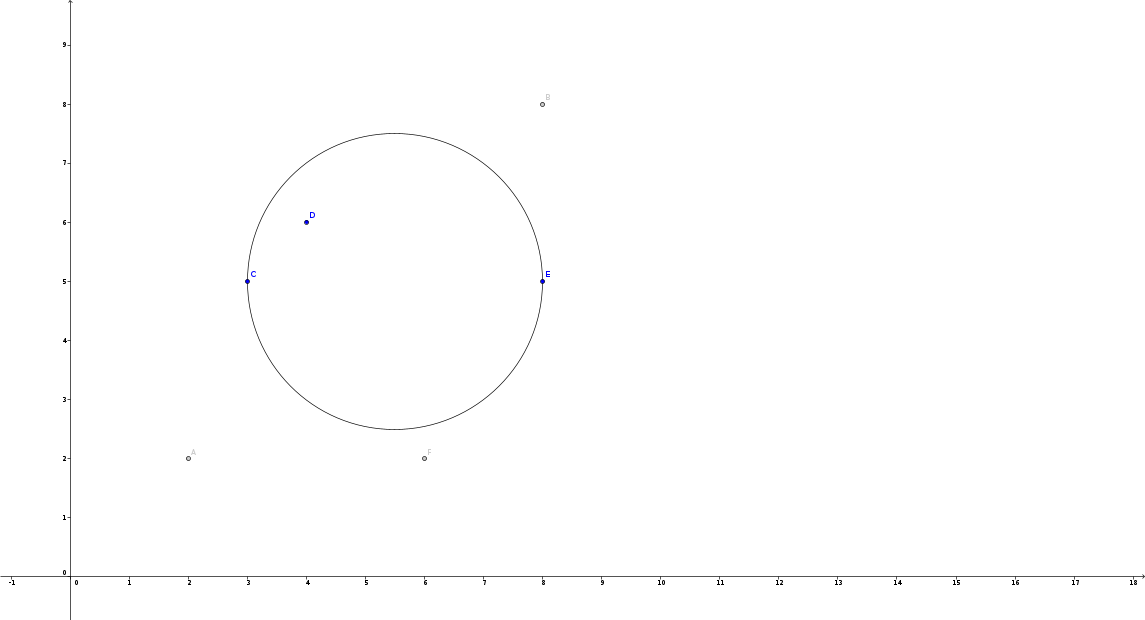
\includegraphics[trim=0 0 7cm 0,clip,width=0.65\textwidth]{figures/SEC05} \\
    $P = \{E, C, D, \mathbf{F}, A, B\}$
\end{frame}
\begin{frame}{Welzl's algorithm...}{Move to the front...}
    \centering
    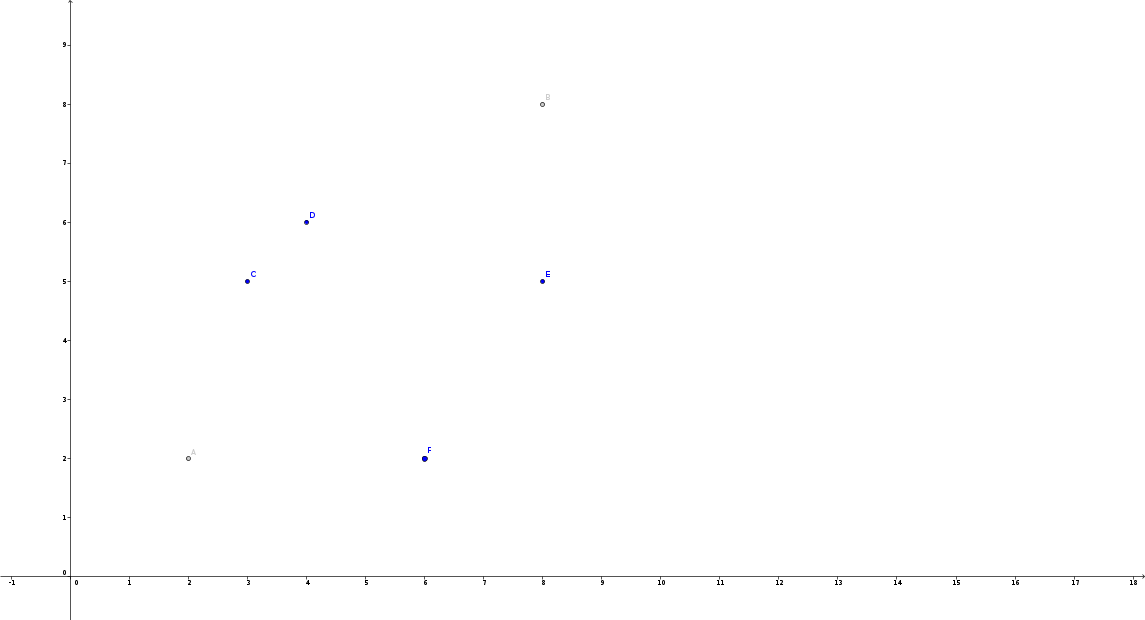
\includegraphics[trim=0 0 7cm 0,clip,width=0.65\textwidth]{figures/SEC06} \\
    $P = \{F, C, E, D, A, B\}$
\end{frame}
\begin{frame}{Welzl's algorithm...}{Find new disk...}
    \centering
    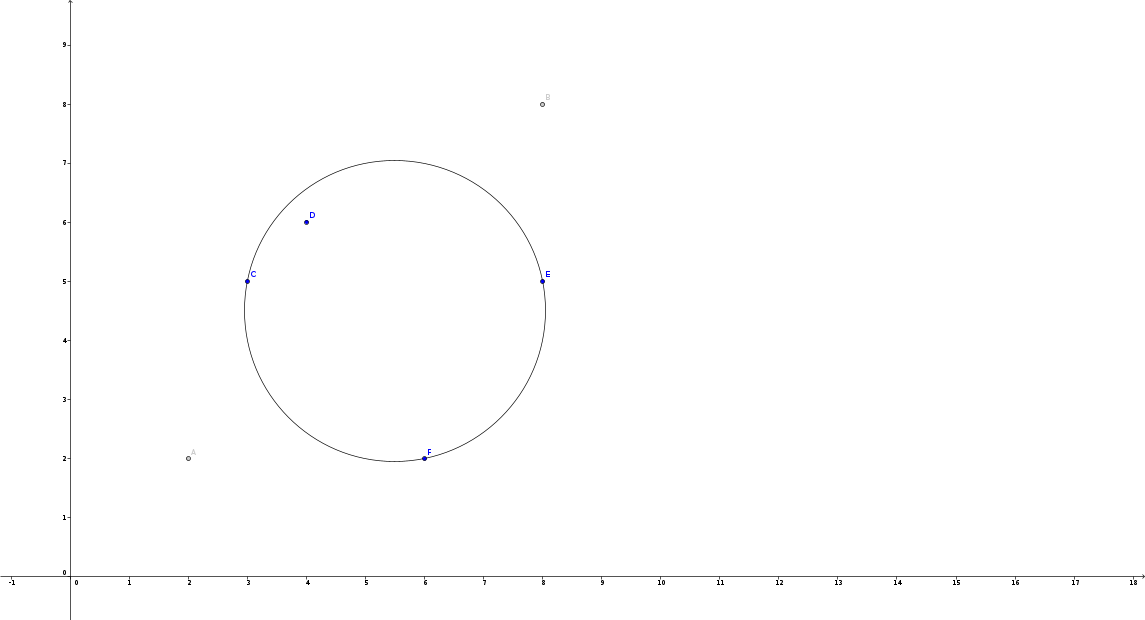
\includegraphics[trim=0 0 7cm 0,clip,width=0.65\textwidth]{figures/SEC07} \\
    $P = \{F, C, E, D, A, B\}$
\end{frame}
\begin{frame}{Welzl's algorithm...}{Query new point...}
    \centering
    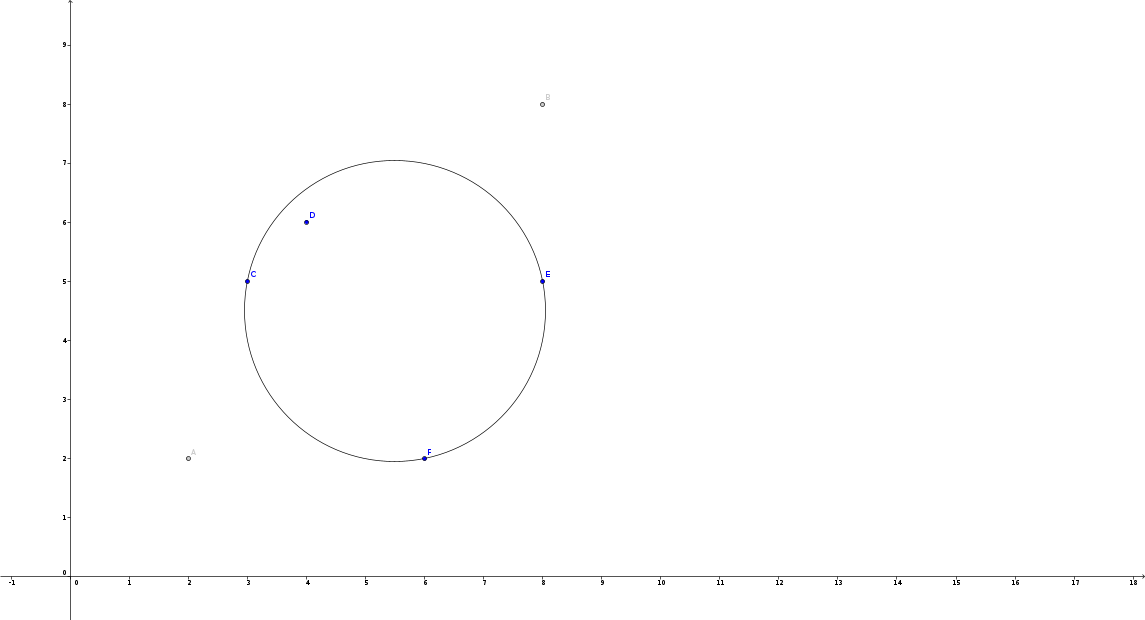
\includegraphics[trim=0 0 7cm 0,clip,width=0.65\textwidth]{figures/SEC07} \\
    $P = \{F, C, E, D, \mathbf{A}, B\}$
\end{frame}
\begin{frame}{Welzl's algorithm...}{Move to the front...}
    \centering
    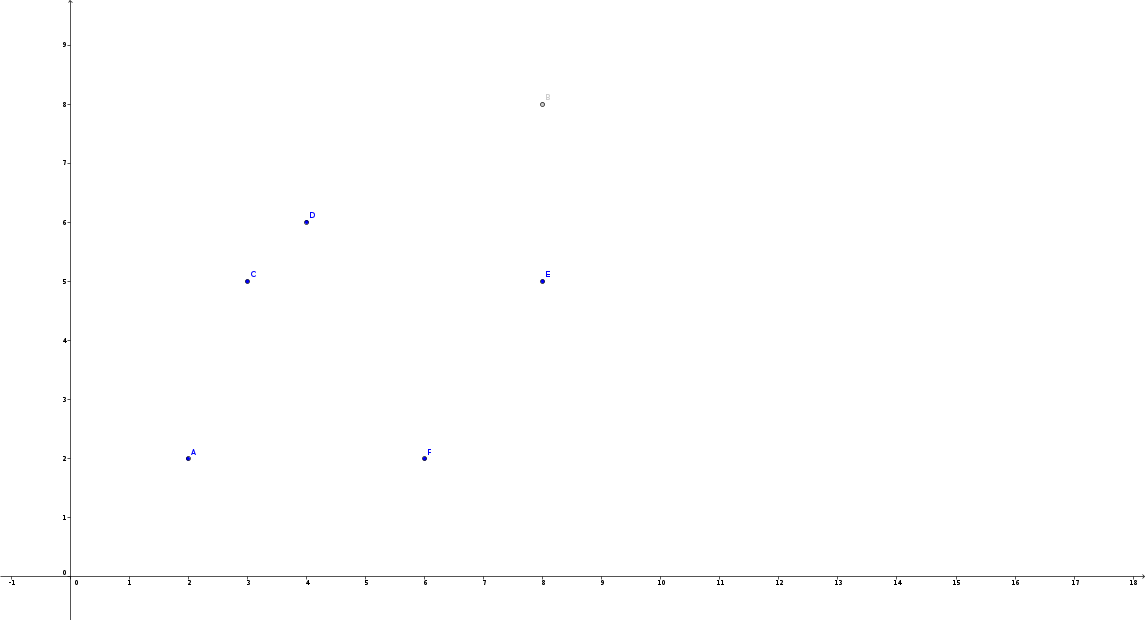
\includegraphics[trim=0 0 7cm 0,clip,width=0.65\textwidth]{figures/SEC08} \\
    $P = \{A, F, C, E, D, B\}$
\end{frame}
\begin{frame}{Welzl's algorithm...}{Find new disk...}
    \centering
    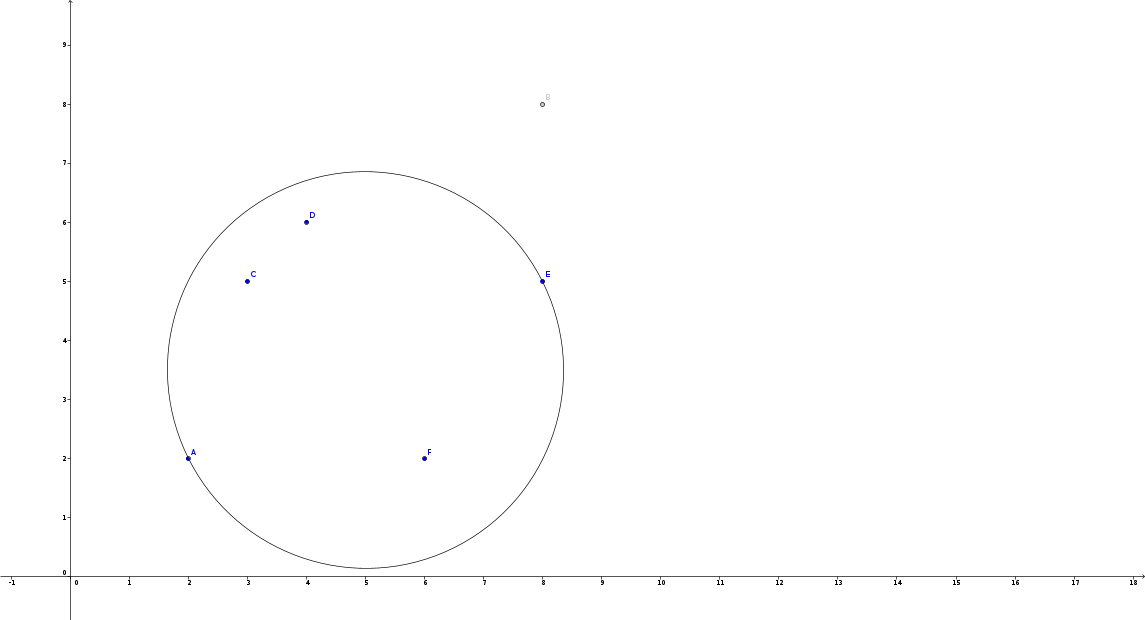
\includegraphics[trim=0 0 7cm 0,clip,width=0.65\textwidth]{figures/SEC09} \\
    $P = \{A, F, C, E, D, B\}$
\end{frame}
\begin{frame}{Welzl's algorithm...}{Query new point...}
    \centering
    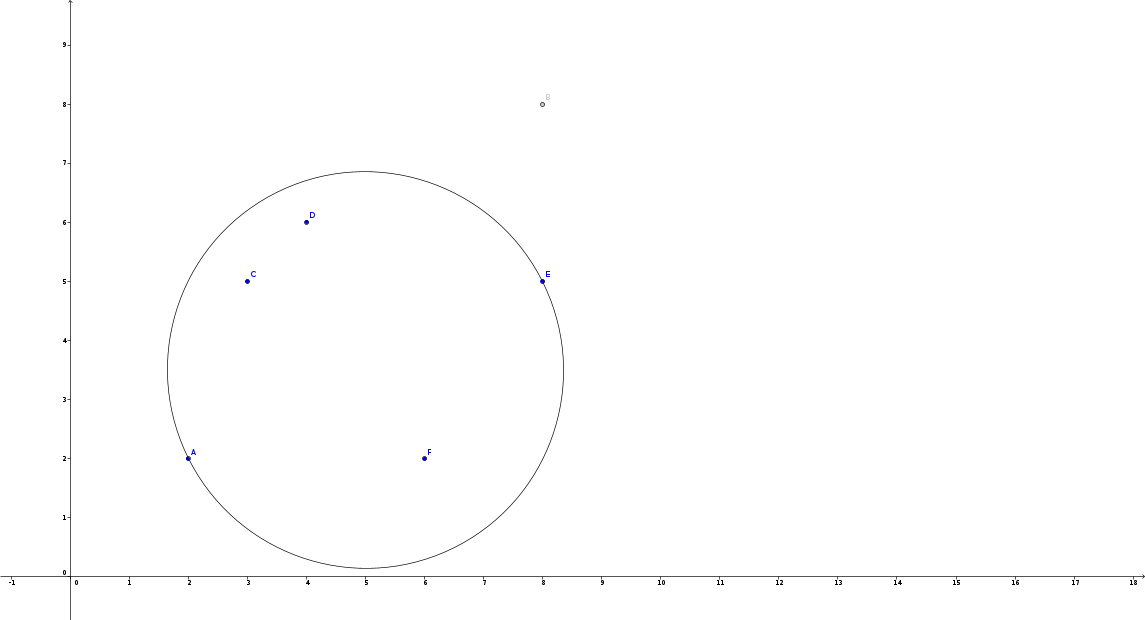
\includegraphics[trim=0 0 7cm 0,clip,width=0.65\textwidth]{figures/SEC09} \\
    $P = \{A, F, C, E, D, \mathbf{B}\}$
\end{frame}
\begin{frame}{Welzl's algorithm...}{Move to the front...}
    \centering
    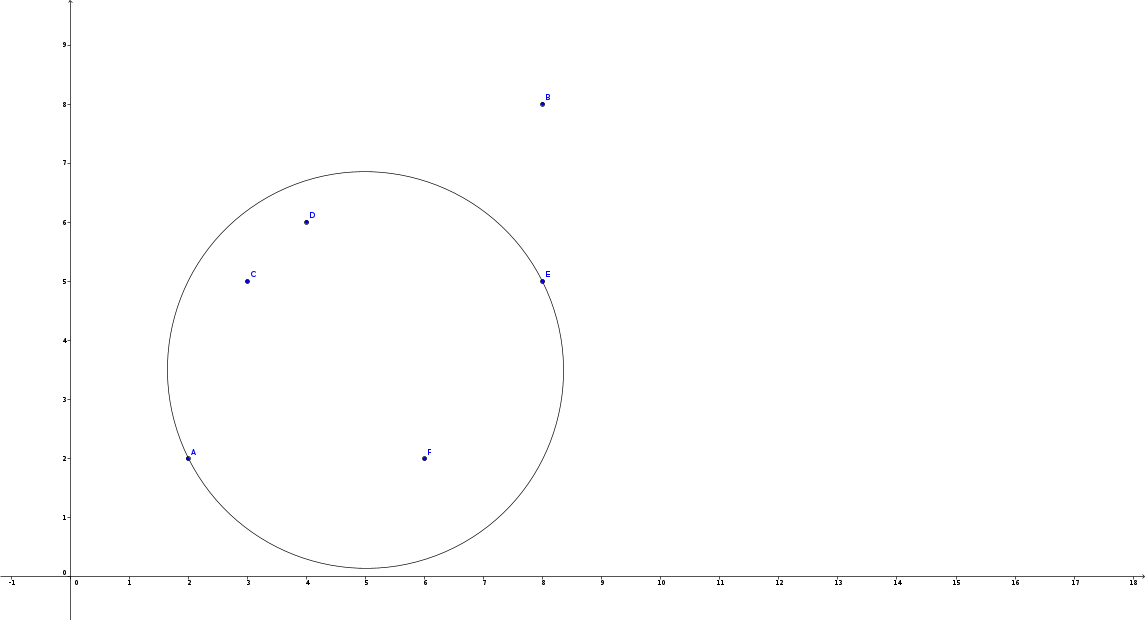
\includegraphics[trim=0 0 7cm 0,clip,width=0.65\textwidth]{figures/SEC10} \\
    $P = \{B, A, E, F, C, D\}$
\end{frame}
\begin{frame}{Welzl's algorithm...}{Finally}
    \centering
    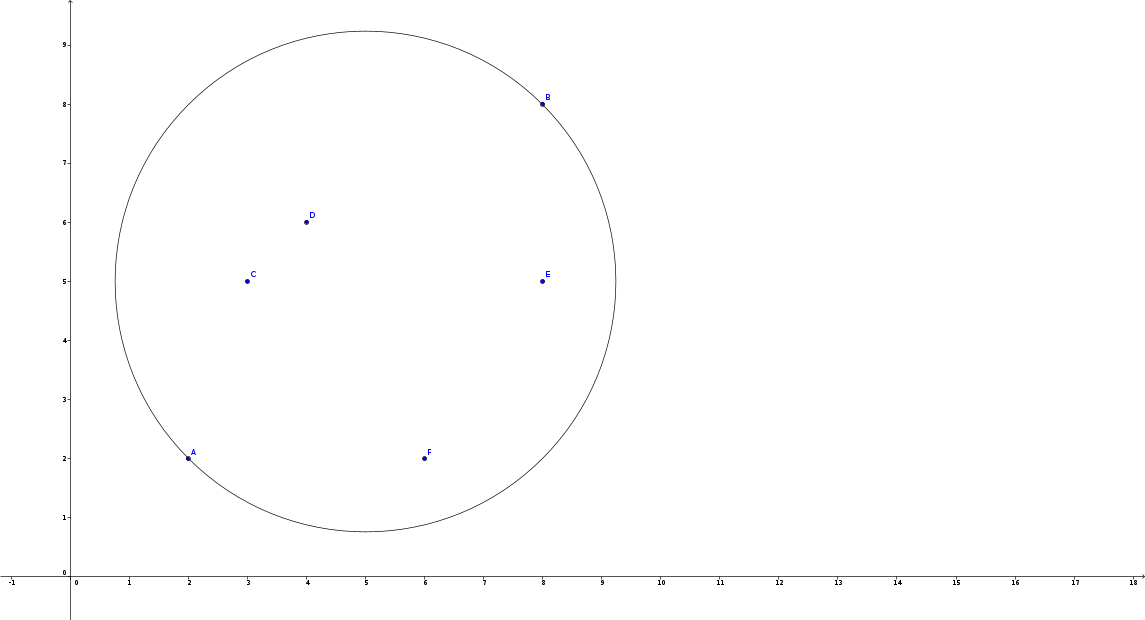
\includegraphics[trim=0 0 7cm 0,clip,width=0.65\textwidth]{figures/SEC11} \\
    $P = \{B, A, E, F, C, D\}$
\end{frame}
\begin{frame}{Welzl's algorithm...}{Expected $O(n)$ complexity }
    \centering
    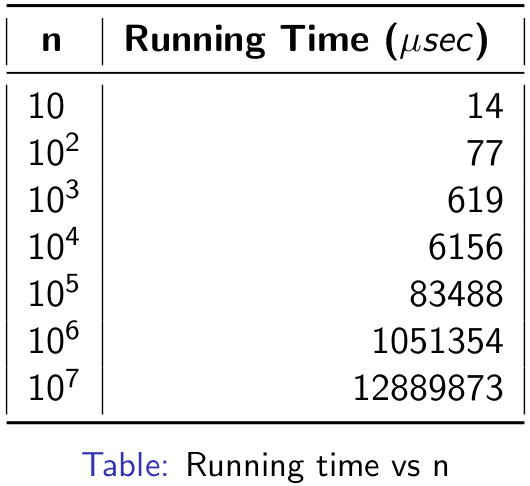
\includegraphics[width=0.33\textwidth]{figures/welzl1} 
    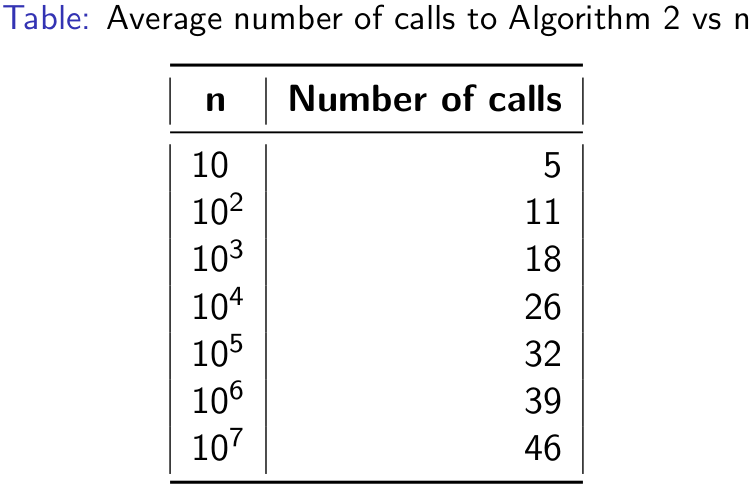
\includegraphics[width=0.55\textwidth]{figures/welzl2} 
    \blfootnote{\tiny{from \url{https://www.cse.iitk.ac.in/users/ssahai/talks/sec.pdf}}}
\end{frame}

\begin{frame}{Adaptation to Flocks - Adding}{Adding a new point}
    \centering
    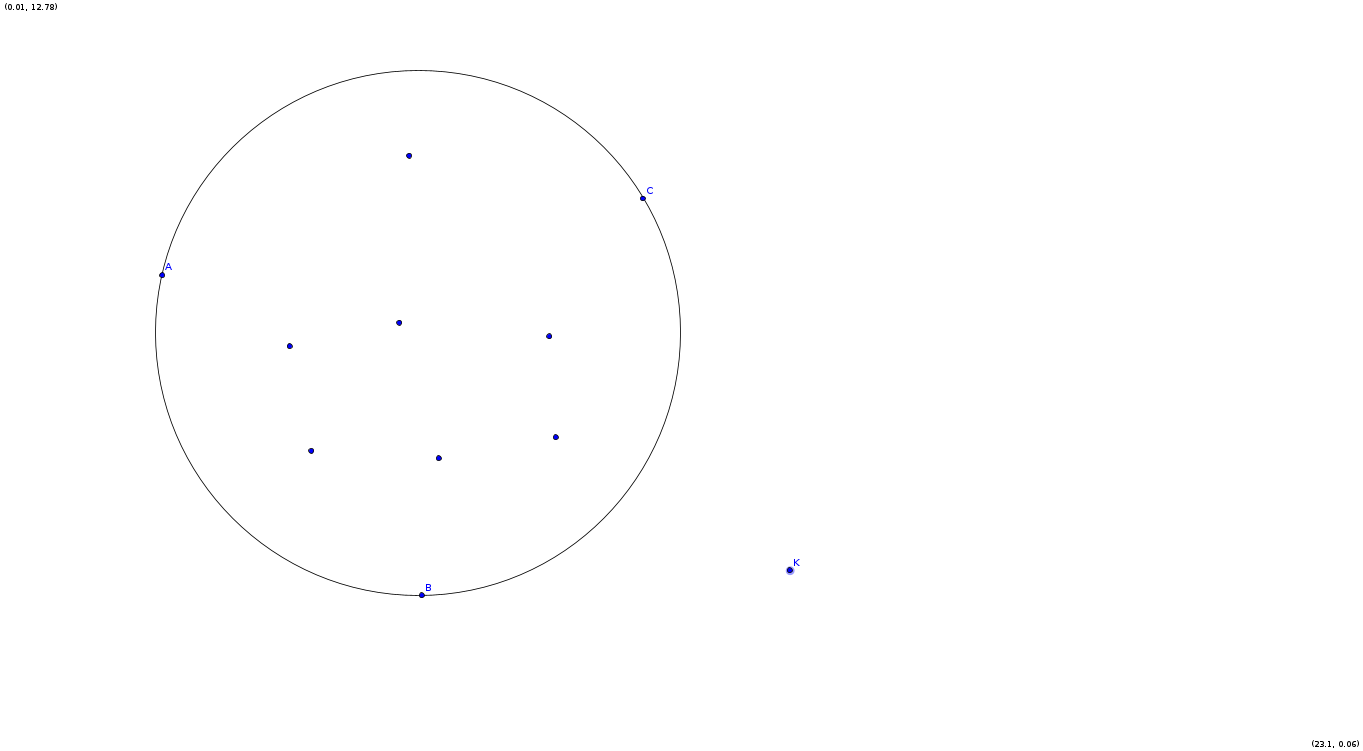
\includegraphics[trim=2cm 0 8cm 0,clip,width=0.65\textwidth]{figures/F01} 
\end{frame}
\begin{frame}{Adaptation to Flocks - Adding}{Keep new point in boundary, remove farthest one...}
    \centering
    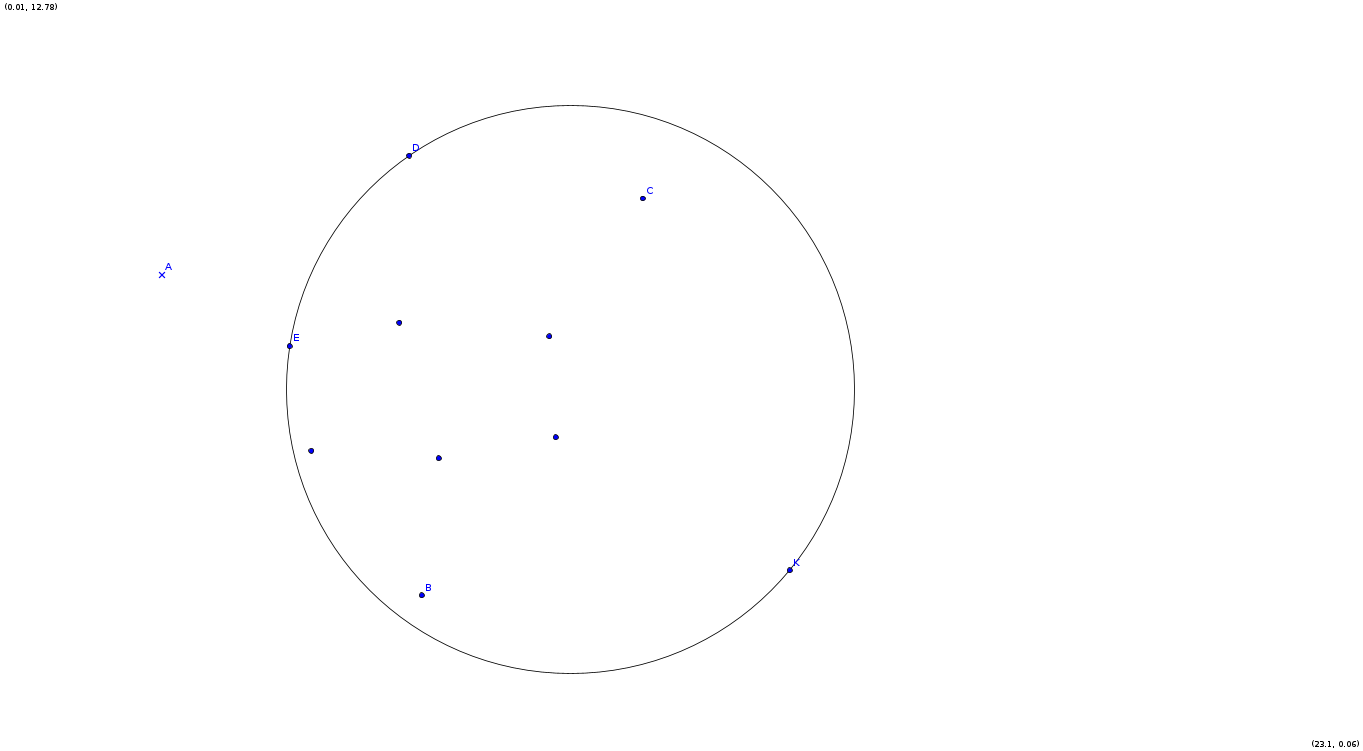
\includegraphics[trim=2cm 0 8cm 0,clip,width=0.65\textwidth]{figures/F02} 
\end{frame}
\begin{frame}{Adaptation to Flocks - Adding}{Repeat until $disk < \varepsilon$...}
    \centering
    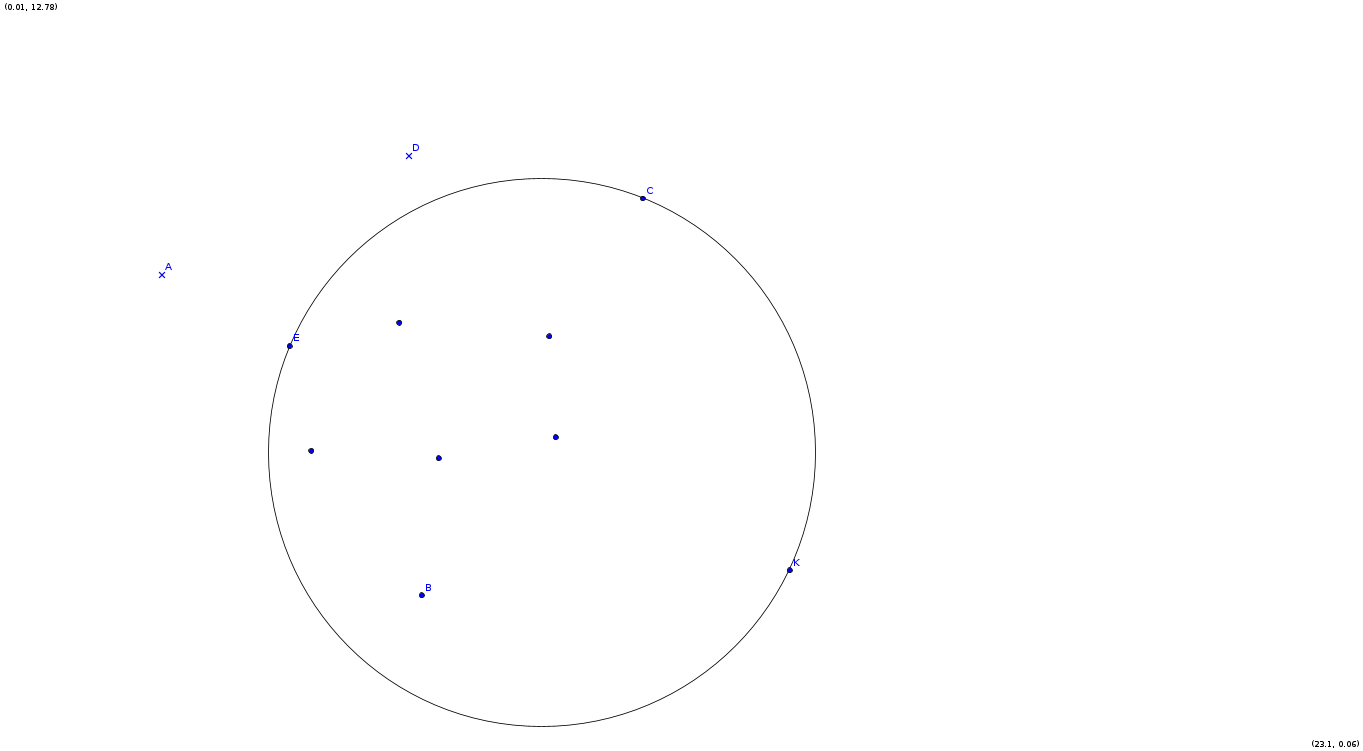
\includegraphics[trim=2cm 0 8cm 0,clip,width=0.65\textwidth]{figures/F03} 
\end{frame}
\begin{frame}{Adaptation to Flocks - Adding}{Find flocks for previous points in boundary...}
    \centering
    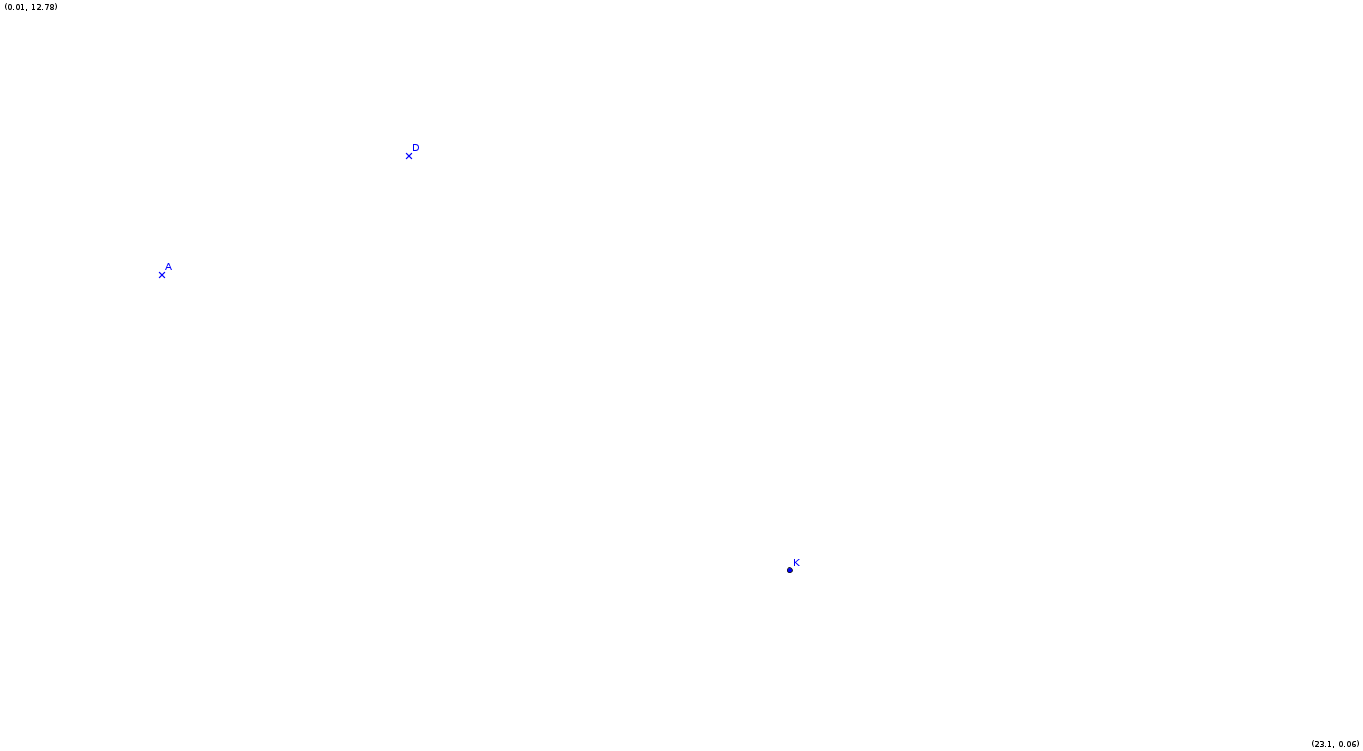
\includegraphics[trim=2cm 0 8cm 0,clip,width=0.65\textwidth]{figures/F04} 
\end{frame}

\begin{frame}{Adaptation to Flocks - Removing}{Identify disk(s) which intersect the point...}
    \centering
    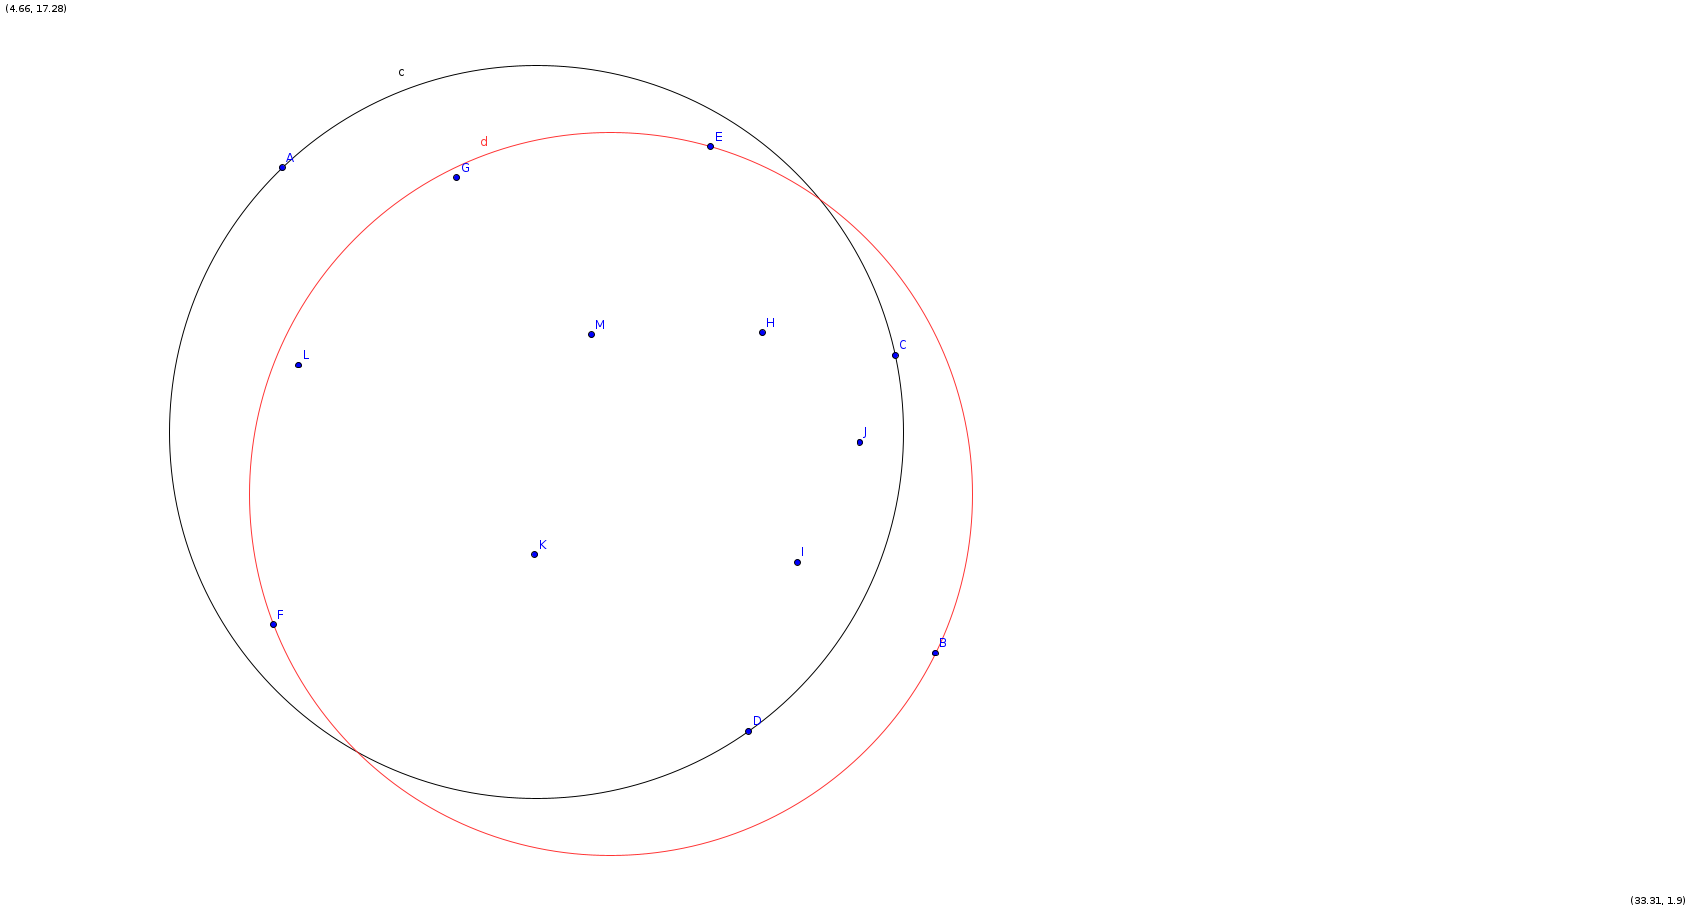
\includegraphics[trim=2cm 0 8cm 0,clip,width=0.65\textwidth]{figures/G01b} 
\end{frame}
\begin{frame}{Adaptation to Flocks - Removing}{Delete point from disk(s)...}
    \centering
    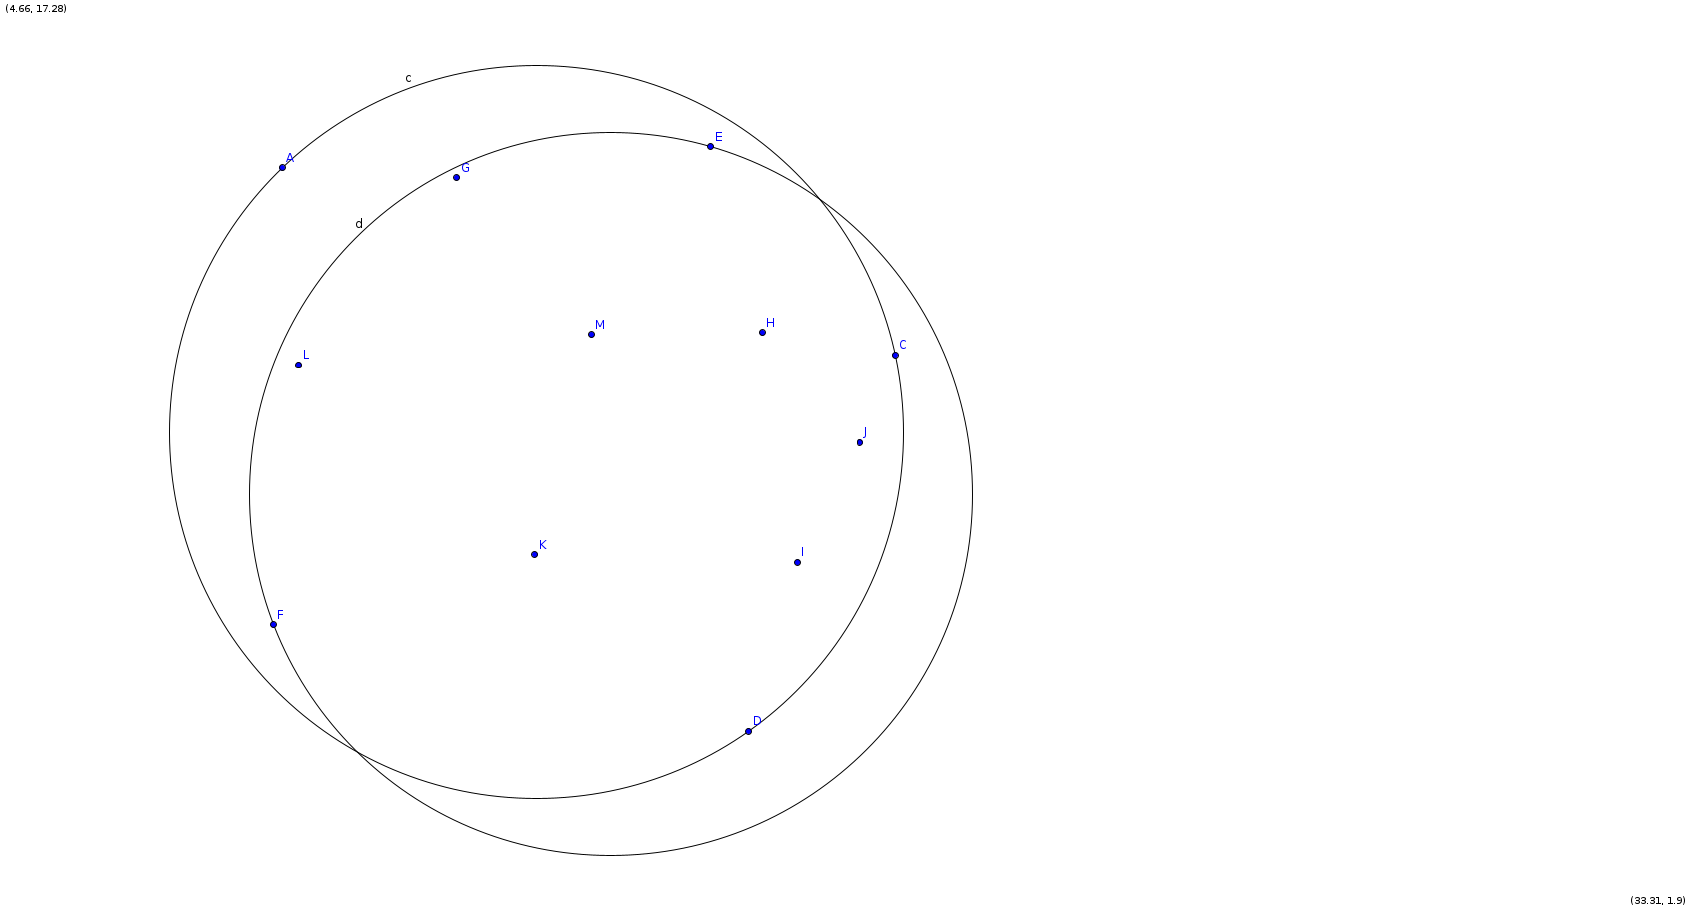
\includegraphics[trim=2cm 0 8cm 0,clip,width=0.65\textwidth]{figures/G02} 
\end{frame}
\begin{frame}{Adaptation to Flocks - Removing}{Prune redundants and duplicates...}
    \centering
    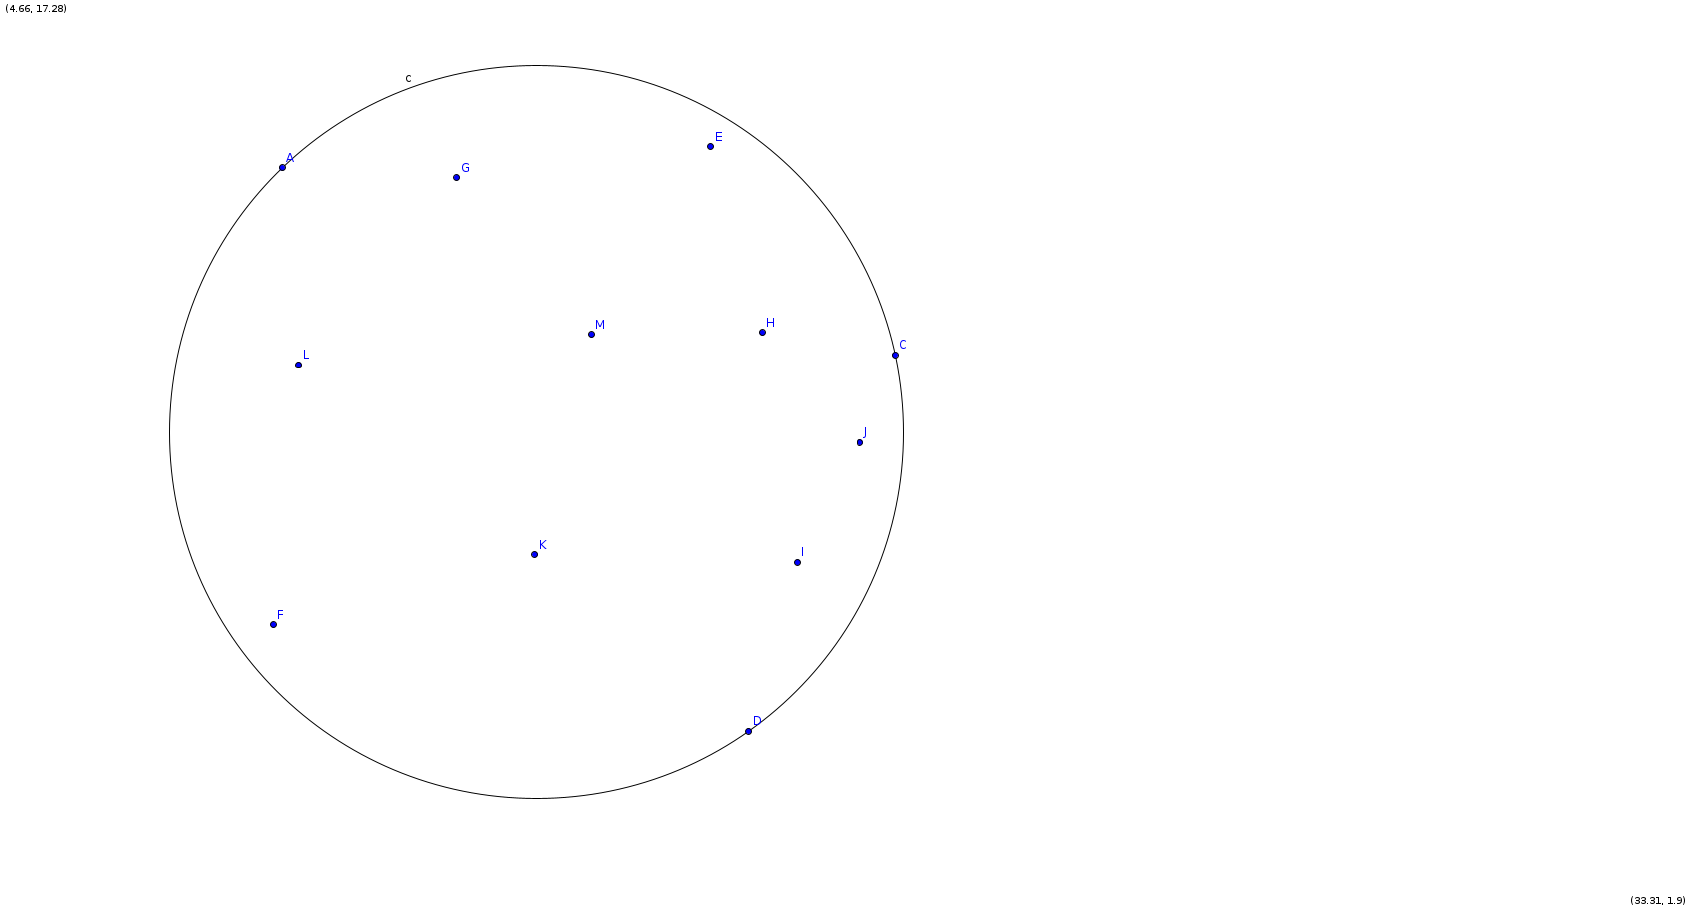
\includegraphics[trim=2cm 0 8cm 0,clip,width=0.65\textwidth]{figures/G03} 
\end{frame}

\end{document}

